\section{Robustness, cross-venue validation, and falsification tests}
\label{sec:robustness}

\subsection{Timestamp alignment, JISDOR averaging window, and alternative FX benchmarks}
A common error in this literature is a fixing-to-close time mismatch (sampling 23:59 UTC crypto against an 08:15 UTC or 09:15 UTC FX benchmark). Panel~A of Table~\ref{tab:robustness} varies synchronization offsets and FX benchmarks systematically. Shifting Indodax and Binance timestamps across $\{-15\text{m}, 0\text{m}, +5\text{m}, +15\text{m}\}$ around the exact BI JISDOR fixing leaves every baseline finding invariant: mean $B_t^{total}$ moves only between $+29.48\text{ bps}$ and $+29.96\text{ bps}$ (SD $79.48$--$80.80\text{ bps}$), mean $B_t^{crypto}$ stays within $[-1.39, -0.83]\text{ bps}$, Engle--Granger $t$-statistics remain below $-4.19$ ($p \le 0.0037$), and Johansen Reinsel--Ahn trace stays tightly grouped between $150.13$ and $153.96$. Next-day JISDOR leads ($N = 1,084$) yield similar point means ($+29.40\text{ bps}$) with slightly higher total basis dispersion ($84.75\text{ bps}$). By contrast, reverting to naive 23:59 UTC crypto closing prices paired against intraday JISDOR inflates pure-crypto dispersion by $31\%$ ($35.97\text{ bps}$ versus $27.44\text{ bps}$) and flips mean $B_t^{crypto}$ sign from $-0.83\text{ bps}$ to $+2.37\text{ bps}$, which measures the size of the timestamp-mismatch bias.

\begin{table}[htbp]
\centering
\caption{Synchronization sensitivity, FX benchmark robustness, and falsification suite (BTC)}
\label{tab:robustness}
\fontsize{6.6}{7.8}\selectfont\setlength{\tabcolsep}{1.6pt}
\begingroup
\begin{tabular}{@{}>{\raggedright\arraybackslash}p{3.0cm}rrrrrrr@{}}
\toprule
\multicolumn{8}{@{}l}{\textbf{Panel A: Timestamp offset, JISDOR-window averaging, and FX benchmark sensitivity}} \\
Specification & $N$ & Mean $B^{tot}$ & SD $B^{tot}$ & Mean $B^{cry}$ & SD $B^{cry}$ & EG $t$ & Trace / Share \\
\midrule
Primary 0m JISDOR & 1,414 & 29.94 & 80.80 & -0.83 & 27.44 & -4.424 & 151.72 \\
Ex-ante $-15\text{m}$ JISDOR & 1,414 & 29.48 & 80.14 & -1.10 & 27.13 & -4.320 & 153.96 \\
Post $+5\text{m}$ JISDOR & 1,414 & 29.96 & 80.43 & -0.95 & 26.69 & -4.419 & 150.13 \\
Post $+15\text{m}$ JISDOR & 1,414 & 29.85 & 79.48 & -1.39 & 26.86 & -4.197 & 150.57 \\
Next-day JISDOR lead & 1,084 & 29.40 & 84.75 & -0.23 & 27.22 & -4.023 & 148.50 \\
23:59 UTC close mismatch & 1,414 & 31.65 & 92.03 & 2.37 & 35.97 & -4.124 & 225.32 \\
Spot FX (Yahoo) 0m & 1,251 & 40.21 & 91.20 & -0.16 & 27.01 & -4.806 & 151.09 \\
ECB FX (Frankfurter) 0m & 1,407 & 30.53 & 81.93 & -0.86 & 27.49 & -4.481 & 158.49 \\
JISDOR-win.\ VWAP (USDT only)$^\dagger$ & 1,414 & 27.06 & 82.87 & -0.83 & 27.44 & -- & 82.4\%$^\dagger$ \\
JISDOR-win.\ VWAP (all 3 legs)$^\dagger$ & 1,414 & 29.64 & 82.65 & 1.75 & 26.65 & -- & 82.8\%$^\dagger$ \\
\midrule
\multicolumn{8}{@{}l}{\textbf{Panel B: Negative controls and falsification tests}} \\
Falsification Test & $N$ & SD (bps) & EG $t$ / $F$ & $p$-val & Trace & Rej.\ 5\% & Expected Outcome \\
\midrule
Omitted FX (BTC/IDR vs.\ USDT) & 1,251 & 669.0 & -1.439 & 0.7839 & 5.81 & No & Fail cointegration \\
Wrong-FX placebo (EUR/USD) & 1,251 & 828.3 & -1.859 & 0.6006 & 6.74 & No & Fail cointegration \\
Cross-asset (BTC/IDR vs.\ XRP$\times$JISDOR) & 1,251 & 3563.3 & -2.467 & 0.2938 & 15.77 & Yes & Mixed (EG fail) \\
30-day time mismatch (BTC) & 1,221 & 2221.1 & -6.451 & $<$0.0001 & 41.87 & Yes & SD explodes \\
Calm-period break (2023-06-15) & 211 & 23.9 & 0.764 & 0.4671 & -- & No & No Chow break \\
\bottomrule
\end{tabular}\endgroup
\begin{minipage}{\textwidth}\footnotesize\vspace{3pt}
\emph{Notes:} $^\dagger$For the two JISDOR monitoring-window VWAP rows, the final column reports the resulting $\mathrm{Var}(B^{s\text{-}FX})/\mathrm{Var}(B^{total})$ share (baseline snapshot share: 83.10\%). The USDT-only VWAP row averages \texttt{USDT/IDR} over each day's exact JISDOR monitoring window while retaining snapshot BTC legs; the all-3-legs VWAP row averages \texttt{BTC/IDR}, \texttt{BTC/USDT}, and \texttt{USDT/IDR} over the monitoring window. In Panel~B, the 30-day mismatch retains algebraic cointegration because a fixed lag of an $I(1)$ price differs by a stationary 30-day return, while destroying tight parity (SD $2,221.1$ vs.\ $80.8\text{ bps}$); the cross-asset placebo fails EG ($p=0.294$) while Trace ($15.77$) marginally exceeds the $15.49$ 5\% CV.
\end{minipage}
\end{table}


A separate concern is that JISDOR is a transaction-weighted average over Bank Indonesia's intraday monitoring window (08:00--16:00 WIB on 920 days, 09:00--15:00 WIB on 432 days, and 08:00--09:45 WIB on 62 days), whereas our baseline samples \texttt{USDT/IDR} at a single five-minute bar at publication time. To check whether averaging-window mismatch inflates $\mathrm{Var}(B_t^{stablecoin\text{-}FX})$, we recompute \texttt{USDT/IDR} as the volume-weighted average (VWAP) and equal-weighted average (TWAP) of all Indodax five-minute bars inside each day's exact JISDOR monitoring window (median 97 bars per day). Matching the averaging window does not reduce stablecoin--FX dispersion: VWAP $B_t^{stablecoin\text{-}FX}$ averages $+27.89\text{ bps}$ with SD $75.22\text{ bps}$ (variance $5,658.51\text{ bps}^2$, or $104.3\%$ of the baseline snapshot variance), leaving the stablecoin--FX share of $\mathrm{Var}(B_t^{total})$ at $82.39\%$ (TWAP $82.47\%$). Volume-averaging all three legs (\texttt{BTC/IDR}, \texttt{BTC/USDT}, and \texttt{USDT/IDR}) over the exact JISDOR monitoring window gives a stablecoin--FX variance share of $82.83\%$ ($B_t^{crypto}$ SD $26.65\text{ bps}$, share $10.39\%$, covariance $6.78\%$; bottom of Table~\ref{tab:robustness}, Panel~A). The $83.1\%$ baseline share is therefore not an averaging-window artifact.

Replacing BI JISDOR with independent FX benchmarks leaves cointegration intact while revealing benchmark-specific level shifts. Pairing Indodax and Binance against ECB/Frankfurter reference rates ($N = 1,407$, SD $81.93\text{ bps}$) produces virtually identical means ($+30.53\text{ bps}$ $B_t^{total}$, $-0.86\text{ bps}$ $B_t^{crypto}$, $\text{Trace}_{RA} = 158.49$). Using continuous Yahoo Finance interbank quotes (\texttt{IDR=X}, $N = 1,251$) preserves exact pure-crypto neutrality ($-0.16\text{ bps}$ mean, $27.01\text{ bps}$ SD) and strong cointegration ($\text{Trace}_{RA} = 151.09$, $p_{boot} \leq 0.0001$), while lifting $B_t^{stablecoin\text{-}FX}$ by roughly $9.6\text{ bps}$ (to $+40.38\text{ bps}$) due to offshore non-deliverable / wholesale quote conventions relative to BI's domestic transaction-weighted JISDOR fixing.

\subsection{Calendar-day versus business-day samples and historical fee uncertainty}
Table~\ref{tab:descriptive} includes calendar-day sensitivity ($N = 2,136$) and closed-FX weekend ($N = 608$) samples to isolate forward-fill distortion. On weekends, carrying Friday's stale JISDOR rate forward inflates $B_t^{total}$ mean and variance ($+34.47\text{ bps}$ mean, SD $86.25\text{ bps}$) solely from weekend global USD/IDR gaps that cannot settle until Monday morning. Throughout those same 608 weekend dates, however, the live domestic \texttt{USDT/IDR} market keeps trading 24/7 alongside offshore crypto, holding BTC $B_t^{crypto}$ centered at $-1.70\text{ bps}$ (SD $27.84\text{ bps}$) with $98.36\%$ two-leg taker band containment. That contrast confirms that apparent weekend rupiah decoupling reflects frozen official FX clocks rather than closed crypto arbitrage.

We also test robustness to two secondary sensitivity dimensions documented in Appendices~\ref{app:provenance} and~\ref{app:details}. First, Table~\ref{tab:lag_sens} varies VECM lag orders ($k \in \{2,\dots,6\}$) and deterministic trend terms (\texttt{det\_order} $\in \{0, 1\}$): rank $r=1$ cointegration holds across all ten models ($\text{Trace}_{RA} = 51.53$ to $201.64$ versus $15.49$ and $18.40$ critical values), global BTC stays weakly exogenous ($p \in [0.191, 0.345]$), and local error-correction speeds stay within $[-0.417, -0.318]$. Second, re-evaluating dynamic cost-band containment across alternative interpretations of the partially verified May 2022--October 2023 Indodax commission cut (Section~\ref{sec:institutional}) moves total BTC $B_t^{crypto}$ containment only modestly around the $98.44\%$ baseline because Regime R2A/R2B all-in Route A taker costs stay within $61.0$--$81.0\text{ bps}$ across either $0/30$ or $10/20$ platform schedules.

\subsection{Direct multi-venue validation against Binance IDR pairs}
To verify that our primary results are not artifacts of an Indodax-specific quote anomaly, Figure~\ref{fig:robustness} compares Indodax directly against Binance's native IDR spot markets (\texttt{BTCIDR} and \texttt{USDTIDR}) across the full $N = 100,362$ five-minute overlap from November 29, 2025 at 12:30 UTC through November 12, 2026 at 23:55 UTC (the longest overlap permitted by Binance's listing date). Over those 349 days, Indodax \texttt{BTC/IDR} averages $-0.19\text{ bps}$ (SD $53.54\text{ bps}$) relative to Binance \texttt{BTC/IDR}, while Indodax \texttt{USDT/IDR} averages $-2.11\text{ bps}$ (SD $25.82\text{ bps}$) relative to Binance \texttt{USDT/IDR}. Cross-venue depth snapshots from November 13, 2026 (Table~\ref{tab:fees} and Figure~\ref{fig:robustness} right panel) explain why price leadership in domestic IDR order flow remains anchored on Indodax: executing a $\$50\text{k}$ round trip incurs $17.99\text{ bps}$ depth spread plus slippage on Indodax \texttt{BTC/IDR} versus $297.38\text{ bps}$ on Binance \texttt{BTC/IDR}, and $5.90\text{ bps}$ versus $22.20\text{ bps}$ on \texttt{USDT/IDR}.

\begin{figure}[htbp]
  \centering
  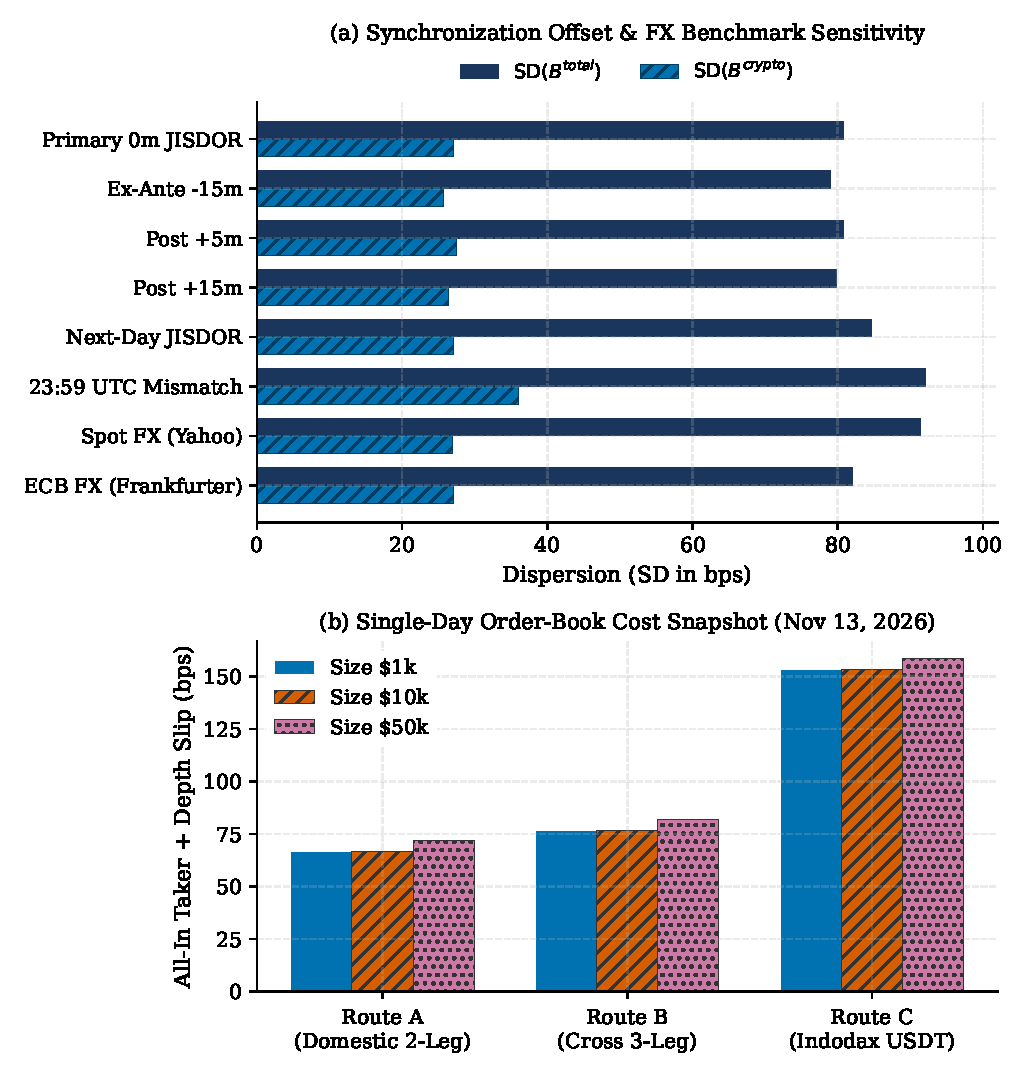
\includegraphics[width=\textwidth]{fig8_robustness_and_orderbook.pdf}
  \caption{Synchronization offset and FX benchmark sensitivity (Panel~a) and live execution cost thresholds by route and trade size from November 13, 2026 limit-order book snapshots (Panel~b).}
  \label{fig:robustness}
\end{figure}

\subsection{Negative controls and falsification suite}
Panel~B of Table~\ref{tab:robustness} reports five negative-control and placebo tests (specified before estimation in the replication code, not in an external registry) ($N = 1,251$ overlapping \texttt{IDR=X} sample for consistent cross-test comparison):
\begin{enumerate}
  \item \textbf{Omitted FX Control:} Regressing $\ln P_t^{IDR}$ on unconverted $\ln P_t^{USDT}$ inflates spread dispersion to $668.99\text{ bps}$ and fails both Engle--Granger ($t = -1.44$, $p = 0.784$) and Johansen ($\text{Trace}_{RA} = 5.81$) cointegration.
  \item \textbf{Wrong-Currency Placebo (\texttt{EUR/USD}):} Substituting euro-dollar FX rates fails to absorb long-run IDR depreciation, blowing spread SD up to $828.32\text{ bps}$ with no cointegration ($t = -1.86$, $p = 0.601$; $\text{Trace}_{RA} = 6.74$).
  \item \textbf{Cross-Asset Placebo (\texttt{BTC/IDR} vs.\ JISDOR-Converted \texttt{XRP/USDT}):} Pairing domestic bitcoin against FX-converted global ripple explodes spread dispersion to $3,563.32\text{ bps}$ ($44\times$ baseline) and fails Engle--Granger cointegration ($t = -2.47$, $p = 0.294$), although bivariate trace sits just above the $5\%$ asymptotic boundary ($15.77$ versus $15.49$) due to shared macro crypto trends over 2021--2026.
  \item \textbf{Deliberate 30-Day Timestamp Mismatch:} Lagging global crypto quotes by 30 calendar days destroys parity completely, inflating spread dispersion to $2,221.11\text{ bps}$ (versus $80.80\text{ bps}$ synchronized) because one-month asset drift overwhelms cross-market arbitrage.
  \item \textbf{Calm Subsample Placebo Break (June 15, 2023):} Testing a Chow structural-break statistic on $B_t^{crypto}$ during the calm 2023 regulatory plateau ($n = 211$) yields $F = 0.764$ ($p = 0.467$), finding no spurious structural break where none occurred.
\end{enumerate}
Collectively, the robustness and falsification checks confirm that documented cointegration, zero-mean pure crypto parity, and dynamic cost containment depend strictly on economically valid currency conversion and genuine intraday time synchronization.
